\documentclass[
paper=128mm:96mm,
fontsize=11pt,
pagesize,
parskip=half-,
]{scrartcl}

\usepackage[nochapters]{classicthesis}

\renewcommand{\sffamily}{\rmfamily}

\usepackage[top=.25in, left=.5in, right=.5in, bottom=.5in]{geometry}
\usepackage{minted}
\newcommand{\slide}[1]{#1 \clearpage}
\newcommand{\sectionslide}[1]{\slide{\hfill \vfill \section{#1}}}

\title{Be A Computer Scientist: Game Programming}
\author{Bendell, XX}
\date{}

\usepackage{graphicx}
\usepackage{eso-pic}

\renewcommand{\baselinestretch}{1.1} 

\renewcommand\maketitle
{
	\vspace*{3ex}
	\begin{center}
		{\Huge Be a Computer Scientist \vspace*{.3em} \par}
		{\large Game Programming \par}
		\vspace*{2em}
	\end{center}
}


\usepackage{titlesec}
\usepackage{multicol}

\titleformat*{\section}{\LARGE}
\titleformat*{\subsection}{\Large}

\titlespacing*{\section}
{0ex}{0ex}{0ex}
\titlespacing*{\subsection}
{0ex}{0ex}{0ex}

\begin{document}
	\AddToShipoutPictureBG{
\includegraphics[height=\paperheight]{gfx/background.jpg}}
	\slide
	{
		\maketitle	
	}
	
	\sectionslide{Presenting Some Bullets}

	\slide
	{
		\subsection{title}
		\begin{itemize}
			\item Really interesting point number 1
			\item Really interesting point number 2
		\end{itemize}
	}
	
	\slide
	{
		{\large Picture here}
		\begin{center}
			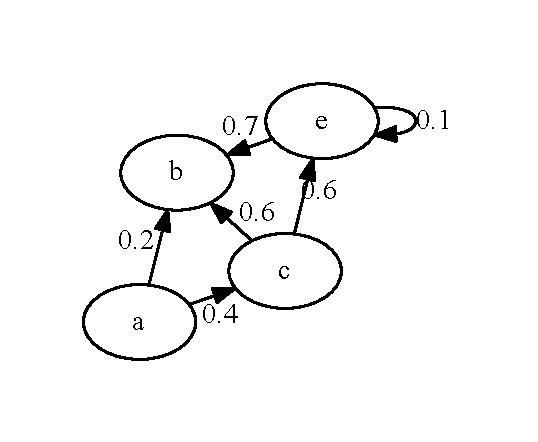
\includegraphics[width=.8\textwidth]{charts/test.pdf}
		\end{center}
	}
	
	\slide
	{
		\subsection{Source Code Listing}
		{
			\footnotesize
			\inputminted{java}{code-snippets/task.java}
		}
	}

	
\end{document}